\section{Carat Data} \label{carat data}

The Carat data consists of samples containing mobile device system settings, current battery level, the list of currently running mobile applications and a user specific identification token unique to each Carat application installation. Each Carat application user periodically sends these samples to the Carat server, typically when the device's battery level changes~\cite{Oliner:2013:CCE:2517351.2517354}. 

Since we are interested about the effects that the mobile devices system settings and state may have on the energy consumption rate of the device, the samples need to be converted in such a way that the energy rate becomes accessible. This was done by grouping all samples according to their user identification token. The grouped tokens were then sorted according to the time of the samples arrival time stamp. These sorted samples were then paired up so that the first sample and the second sample make up pair number 1, the second and the third sample make up sample pair number 2 and so forth. These sample pairs were used as the basis of this analysis. The energy rate of a sample pair was calculated as the difference of the samples' battery levels divided by the difference of their time stamps. The set of running applications for a sample pair was decided to be the union of both samples running applications. For all other system settings and state the more recent sample of the pair was used to determine the state or settings of the sample pair.

Since the Carat data comes from a large number of unsupervised clients, there is no guarantee for the integrity of the data. A faulty device or a hostile client may produce erroneous data. It is therefore essential to apply filtering to the data to minimize the amount of erroneous data. 

Let us give a brief description of each of the system settings and state variables that were used as part of the analysis. Association analysis requires discrete data, as explained in chapter~\ref{association analysis}. Therefore we describe the way each of these variables is discretized. The following presentation of the data is based on a subset of the Carat data consisting of samples that were collected between 26.8.2016 and 3.10.2016 that had Facebook mobile application running. For increased uniformity and simplicity, the data set only contains samples from clients running Android operating system. 

\subsection{Energy Rate}

Energy rate of a mobile device is the velocity at which the mobile devices battery is discharging. The unit of the energy rate is percentage per second. This means that an energy rate of $\frac{0.05}{s}$ would drain the whole battery in just $\frac{100}{0.05 / s} = 2000 s \approx 33 minutes$.

\begin{figure}[!htbp]
	\centering
	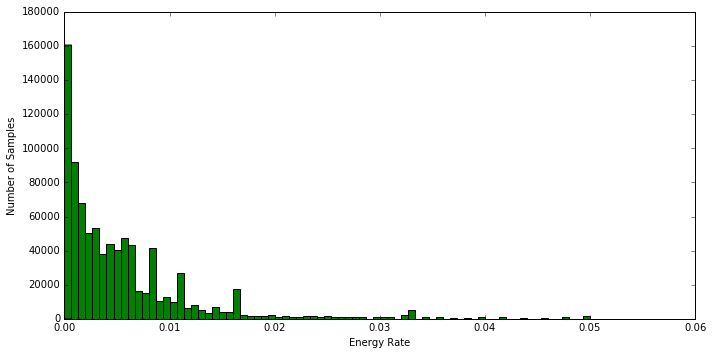
\includegraphics[width=\textwidth]{images/carat-data/energy_rate.png}
	\caption{Histogram of energy rates with 75 bins}
	\label{figure:carat-data-energy-rate}
\end{figure}  

Figure~\ref{figure:carat-data-energy-rate} shows a histogram of the energy rate distribution. The distribution appears to be a rough approximation of an exponential distribution. The distribution does not seem have an evident categorical division. Thus, the data was discretized by dividing it to four bins of equal frequency. 

\subsection{CPU Usage Level}  

CPU usage level is the fraction of time that the central processing unit(s) of the mobile device were busy when the sample was collected. The CPU usage level is in a unit of percentages of the maximum level. All CPU usage levels that were below zero or greater than 100 were discarded as faulty data.

\begin{figure}[!htbp]
	\centering
	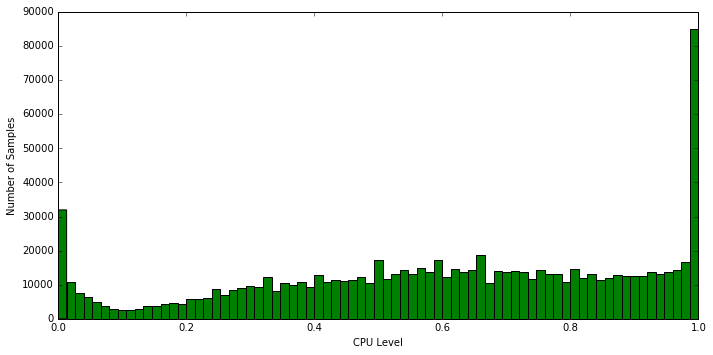
\includegraphics[width=\textwidth]{images/carat-data/cpu_level.png}
	\caption{Histogram of CPU usage levels with 75 bins}
	\label{figure:carat-data-cpu-level}
\end{figure}  

Figure~\ref{figure:carat-data-cpu-level} shows a histogram of the CPU usage level distribution. The distribution very roughly approximates the uniform distribution except for 100\% and 0\% CPU usage levels, which are quite overrepresented. The data was discretized into four bins of equal frequency.

One would assume that higher CPU usage levels lead to higher energy rates. 

\subsection{Travel Distance}  

Travel distance is the distance in meters, that the mobile device moved between the two samples. 

\begin{figure}[!htbp]
	\centering
	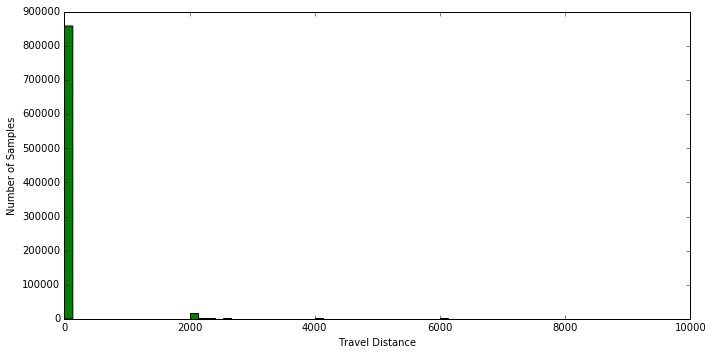
\includegraphics[width=\textwidth]{images/carat-data/travel_distance.png}
	\caption{Histogram of travel distance with 75 bins}
	\label{figure:carat-data-travel-distance}
\end{figure}  

Figure~\ref{figure:carat-data-travel-distance} shows a histogram of the travel distance distribution. Most of the mass of the distribution is concentrated in the close proximity of zero with other values having very low frequencies. The travel distance was discretized to two categories: \textit{moving}, if the travelled distance was greater than 100 meters, and \textit{static} otherwise.

\subsection{Battery Temperature}  

Battery temperature is the measured mobile device battery temperature in degrees Celsius. Temperatures smaller than five degrees were discarded as it is very rare for a battery temperature to be that low even in subzero climates. Likewise battery temperatures of over 100 degrees were discarded, as healthy devices very rarely reach such high battery temperatures.

\begin{figure}[!htbp]
	\centering
	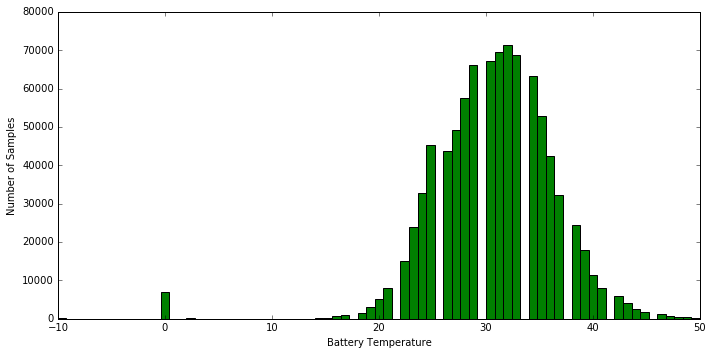
\includegraphics[width=\textwidth]{images/carat-data/battery_temperature.png}
	\caption{Histogram of battery temperatures with 75 bins}
	\label{figure:carat-data-battery-temperature}
\end{figure}  

Figure~\ref{figure:carat-data-battery-temperature} shows a histogram of the battery temperature distribution. The distribution approximates a normal distribution with some skewedness. Notably, there is a small cluster of measurements near zero degrees Celsius. This is most likely due to mobile devices systematically reporting a value of zero if the measurement data is not available. The data was discretized into four bins of equal frequency.

A straightforward hypothesis would be that a higher battery temperature leads to increased energy rate.

\subsection{Battery Voltage}  

Battery voltage is the electric potential difference generated by the battery in units of volts.

\begin{figure}[!htbp]
	\centering
	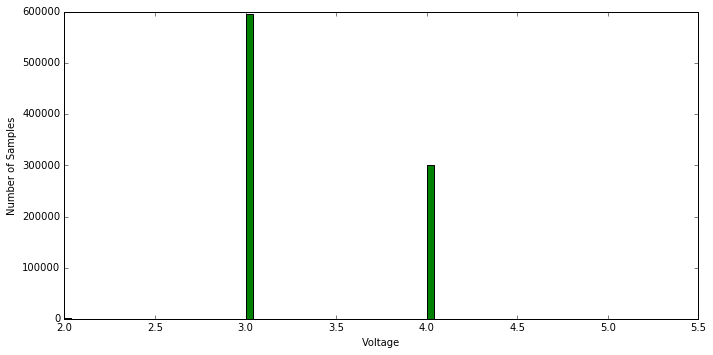
\includegraphics[width=\textwidth]{images/carat-data/battery_voltage.png}
	\caption{Histogram of battery voltages with 75 bins}
	\label{figure:carat-data-battery-voltage}
\end{figure}  

Figure~\ref{figure:carat-data-battery-voltage} shows a histogram of battery voltage distribution from the Carat data. The voltages are clustered almost discretely around values of 2, 3 and 4 volts. The voltages were divided to three bins of equal mass to reflect this clustering.    

\subsection{Screen Brightness}  

Screen brightness is system setting that takes integer values between -1 and 255. Higher values correspond to higher screen brightness. The value negative one has a special meaning indicating automatic screen brightness, where the screen's brightness is adjusted according to changing illumination of the environment~\cite{PELTONEN201671}.

\begin{figure}[!htbp]
	\centering
	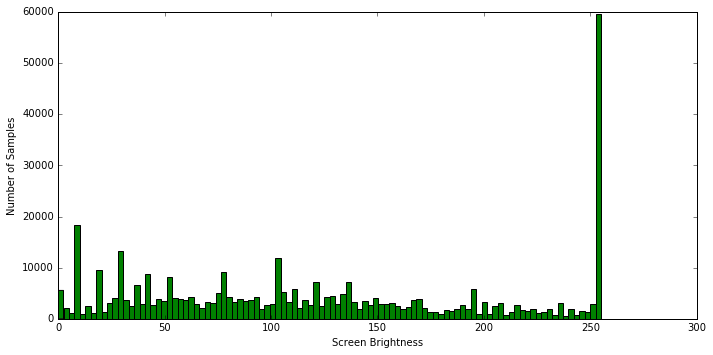
\includegraphics[width=\textwidth]{images/carat-data/screen_brightness.png}
	\caption{Histogram of screen brightness divided to 100 bins}
	\label{figure:carat-data-screen-brightness}
\end{figure}    

Figure~\ref{figure:carat-data-screen-brightness} shows a histogram of the screen brightness values, where the values of -1 have been removed. The brightness values seem to roughly follow a uniform distribution, although very high screen brightness settings seem to be over represented. Approximately half of the samples had their brightness value at -1, indicating automatic brightness setting. Since the automatic setting is categorically different from all other brightness values, the brightness attribute was discretized in the following way: the value -1 formed it's own bin and the numerical values were divided to four bins of equal mass.   

A very intuitive hypothesis would be that the screen brightness is a large factor in the overall energy rate of any mobile device.

\subsection{Mobile Network Technology}  

The mobile network technology is a system property that reports the name of the mobile technology that mobile device is using for its mobile data communication. These 

\begin{figure}[!htbp]
	\centering
	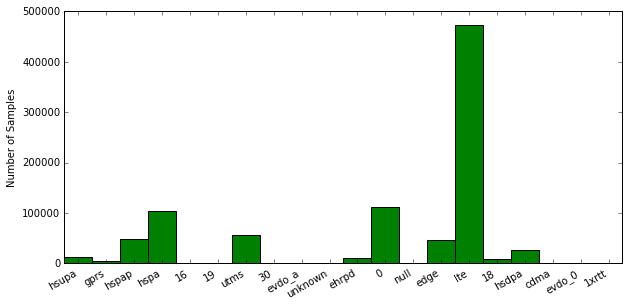
\includegraphics[width=\textwidth]{images/carat-data/mobile_net_type.png}
	\caption{Histogram of mobile network technologies in Carat data}
	\label{figure:carat-data-mobile-net-type}
\end{figure}   

Figure~\ref{figure:carat-data-mobile-net-type} shows a histogram of all mobile network types in the Carat data. Ambiguous categories of "16", "19", "30", "unknown", "null" and "18" were combined to a single bin labelled as "unknown".

Intuitively, one would assume that older mobile network technologies such as \textit{gprs} would consume less battery life than newer technologies such as \textit{lte}, since the newer technologies achieve much greater data rates than the old technologies.

\subsection{Network Type}  

Network type is the system property that the is reported by the mobile device to indicate the type data connection. Typically this is either \textit{mobile} or \textit{wifi}, indicating the use of mobile networking or a wireless local area networking respectively. Some more exotic alternatives can however be found in the data, such as \textit{bluetooth tethering}, where the network access is enabled by bluetooth tunneling through another device.

\begin{figure}[!htbp]
	\centering
	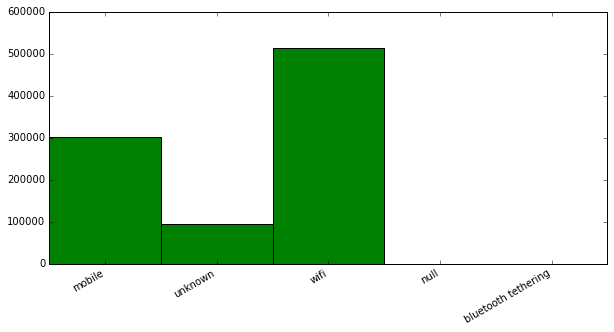
\includegraphics[width=\textwidth]{images/carat-data/network_type.png}
	\caption{Histogram of network types in Carat data}
	\label{figure:carat-data-net-type}
\end{figure}   

Figure~\ref{figure:carat-data-net-type} shows a histogram of all network types found in the Carat data. Values \textit{null} and \textit{unknown} were considered ambiguous and were combined under the label \textit{unknown}.
 

\subsection{WiFi Signal Strength}

WiFi signal strength is a system property that the mobile device uses to signify the strength of the wireless local area network. WiFi connection strength is reported as an integer value in the range -100 to 0, where 0 signifies the strongest signal. Presumably, the WiFi signal strength is in units of decibels relative to milliwatt (dBm). The Android API seems to report a value of -127 when no reading is available. Values less than -100 were excluded from the data as these are very unlikely to be real measurements.

 \begin{figure}[!htbp]
	\centering
	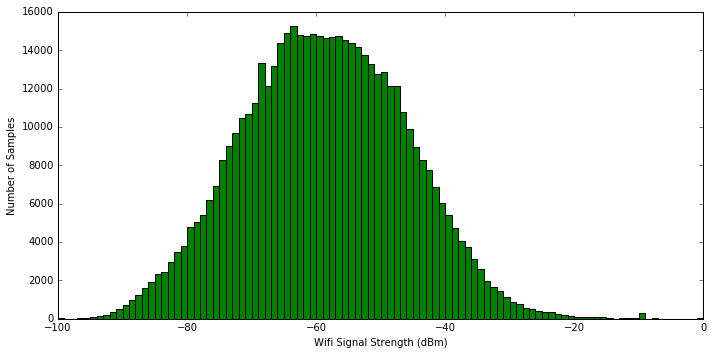
\includegraphics[width=\textwidth]{images/carat-data/wifi_signal_strength.png}
	\caption{Histogram of WiFi signal strengths readings with 100 bins in Carat data}
	\label{figure:carat-data-wifi-signal-strength}
\end{figure} 

Figure~\ref{figure:carat-data-wifi-signal-strength} shows a histogram of WiFi signal strengths in Carat data. The distribution seems to approximate a normal distribution reasonably well. 

One hypothesis for the interactions between the signal strength and energy rate would be that lower signal strength leads to higher energy rate, as low signal strength s generally increase the noisiness of the connection, leading to increased data loss and retransmissions, which require extra battery life.

\subsection{WiFi Connection Speed}

WiFi Connection speed is a system property that the mobile device uses to report the current wireless local area network link speed. The link speed is presumably reported in units of mega bits per second (mbps). 

A reasonable hypothesis for the WiFi connection speed - energy rate -interaction would be that higher speed is related to higher energy rate, since wireless communication is quite energy intensive. 

 \begin{figure}[!htbp]
	\centering
	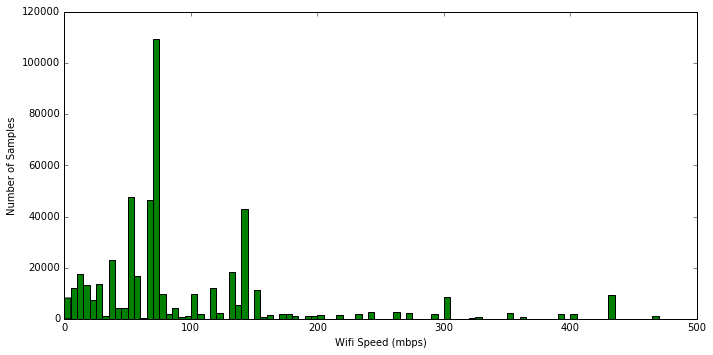
\includegraphics[width=\textwidth]{images/carat-data/wifi_speed.png}
	\caption{Histogram of WiFi link speed with 100 bins in Carat data}
	\label{figure:carat-data-wifi-speed}
\end{figure}

Figure~\ref{figure:carat-data-wifi-speed} shows a histogram of the WiFi speeds in the Carat data. 